\documentclass[paper=a4, fontsize=11pt]{article}

\usepackage{amsmath,amsfonts,amsthm,graphicx} % Math packages
\usepackage[explicit]{titlesec}
\usepackage{fancyhdr} % Custom headers and footers
\usepackage[super]{nth}
\usepackage{parskip}
\usepackage{commath}
\usepackage{amssymb}
\usepackage{mathtools}
\usepackage{enumitem}
\usepackage{textcomp}
\usepackage{wrapfig, framed, caption}
\usepackage{nicefrac}
\usepackage{booktabs,float,siunitx}
\usepackage{subcaption}
\usepackage{bbm}
\usepackage{titling}
\usepackage{multirow}
\usepackage{hyperref}
\usepackage{wrapfig}
\usepackage{forest}
\preauthor{\begin{flushright}\Large}
\postauthor{\par\end{flushright}}

\usepackage{color} %red, green, blue, yellow, cyan, magenta, black, white
\usepackage[margin=0.7in]{geometry}
\usepackage{pdflscape}
\usepackage{changepage}



%\usepackage [utf8]{inputenc}
%\usepackage[x11names]{xcolor}
%\usepackage[overload]{empheq}
%\colorlet{textcolor}{black}
%\usepackage{listings}
%\usepackage{sectsty} % Allows customizing section commands
%\usepackage{graphicx}
%\usepackage{caption}
%\usepackage{graphicx} 

\newcommand*{\widebox}[2][0.5em]{\fbox{\hspace{#1}$\displaystyle #2$\hspace{#1}}}

\makeatletter
\newcommand*{\centerfloat}{%
  \parindent \z@
  \leftskip \z@ \@plus 1fil \@minus \textwidth
  \rightskip\leftskip
  \parfillskip \z@skip}
\makeatother


%\definecolor{mygreen}{RGB}{28,172,0} % color values Red, Green, Blue
%\definecolor{mylilas}{RGB}{170,55,241}

\def\du#1{\underline{\underline{#1}}}

\pagestyle{fancyplain} % Makes all pages in the document conform to the custom headers and footers
\fancyhead{} % No page header - if you want one, create it in the same way as the footers below
\fancyfoot[L]{} % Empty left footer
\fancyfoot[C]{} % Empty center footer
%\fancyfoot[R]{\thepage} % Page numbering for right footer
\renewcommand{\headrulewidth}{0pt} % Remove header underlines
\renewcommand{\footrulewidth}{0pt} % Remove footer underlines
\setlength{\headheight}{8pt} % Customize the height of the header

%\numberwithin{equation}{section} % Number equations within sections (i.e. 1.1, 1.2, 2.1, 2.2 instead of 1, 2, 3, 4)
%\numberwithin{figure}{section} % Number figures within sections (i.e. 1.1, 1.2, 2.1, 2.2 instead of 1, 2, 3, 4)
%\numberwithin{table}{section} % Number tables within sections (i.e. 1.1, 1.2, 2.1, 2.2 instead of 1, 2, 3, 4)

\setlength\parindent{0pt} % Removes all indentation from paragraphs - comment this line for an assignment with lots of text

%\titleformat{\section}{\normalfont\Large\bfseries}{}{0em}{#1}


%\renewcommand\thesubsection{\alph{subsection}}


%----------------------------------------------------------------------------------------
%	TITLE SECTION
%----------------------------------------------------------------------------------------

\newcommand{\horrule}[1]{\rule{\linewidth}{#1}} % Create horizontal rule command with 1 argument of height

\newcommand{\mychar}[1]{%
  \begingroup\normalfont
  \includegraphics[height=0.8em]{#1}%
  \endgroup
}

%\newcommand{\abs}[1]{\left\lvert#1\right\rvert}

\definecolor{fblue}{RGB}{92,144,192}
\definecolor{fgreen}{RGB}{34,162,70}

\newcommand\myfolder[2][fblue]{%
\begin{tikzpicture}[overlay]
\begin{scope}[xshift=20pt]
\filldraw[rounded corners=1pt,fill=#1,draw=white,double=black]
  (-23pt,10pt) -- ++(3pt,5pt) -- ++(18pt,0pt) -- ++(40:3pt) -- ++(9pt,0pt) -- ++(-40:3pt)
  -- (20pt,15pt) -- (23pt,10pt) -- cycle;
\filldraw[rounded corners,draw=white,double=black,top color=#1,bottom color=#1!30]
  (-22pt,-12pt) -- ++(44pt,0pt) -- (25pt,12pt) coordinate (topr) -- ++(-50pt,0pt) coordinate (topl) -- cycle;
\end{scope}  
\end{tikzpicture}%
\makebox[40pt]{\raisebox{-3pt}{{\footnotesize\ttfamily#2}}}%
}
\newcommand\myfile[2][fblue]{%
{\footnotesize\ttfamily#2}%
}

\newcommand*\circled[1]{\tikz[baseline=(char.base)]{
            \node[shape=circle,draw,inner sep=0.4pt] (char) {#1};}}

\title{	
\normalfont \normalsize \vspace{-1cm}
\textsc{ECE4053: Power System Analysis} \\ [14pt]
\horrule{0.5pt} \\[0.1cm]
\huge Lab 2 - Intro to PSS/E continued \\
\horrule{2pt} \\[0.2cm]
}
\author{}
\date{}

\begin{document}

\maketitle

%----------------------------------------------------------------------------------------
%	QUESTION 1
%----------------------------------------------------------------------------------------
\vspace{-1.5cm}
\section{Recap}
Hopefully from last week we remember:
\begin{itemize}
\item{Navigating the PSS/E GUI}
\item{Opening a saved case}
\item{Creating and saving a saved case}
\end{itemize}

\section{Goals for this lab}
The main two goals for this lab are:
\begin{itemize}
\item{Performing a load flow using PSS/E}
\item{Exporting results}
\end{itemize}

\section{Simulation files}
Please download \texttt{Lab2\_files.zip} from Moodle and extract the contents onto your hard drive. You should have the following file structure:

\begin{figure} [h]
\centering
\begin{forest}
	for tree={
		font=\sffamily,
		grow'=0,
		inner ysep=12pt,
		child anchor=west,
		parent anchor=south,
		anchor=west,
		calign=first,
		edge=densely dotted,
		edge path={
			\noexpand\path [draw, \forestoption{edge}]
			(!u.south west) +(12.5pt,0) |- (.child anchor)\forestoption{edge label};
		},
		before typesetting nodes={if n=1 {insert before={[,phantom,minimum height=18pt]}} {}},
		fit=band,
		before computing xy={l=25pt},
		for children={s sep-=0.8em}
	}
[{\myfolder[fgreen]{Lab2\_files}}
    [{\myfile{Lab2.sav}}]
    [{\myfile{Lab2.sld}}]
]
\end{forest}
\end{figure}

\section{Problem description}
The \texttt{Lab2.sav} file is a saved case of the network we were entering last week in Task B. For completeness we provide the same summary here:

\begin{quote}
A substation ``Metro'' in a metropolitan area in a remote mining area supplies the town load by 132/33kV transformers and loads at 132kV for the mine at the town, ``Mine A'' and a plant for processing of minerals, ``MinProc''. ``Metro'' is supplied at 132kV by a 30 km double circuit line from the gas power station ``Gas'' and by a 100km double circuit 132 kV line from a hydro power station ``Hydro''. ``Mine A'' has a continuous load of 50MW, MinProc has a continuous load of 100MW and the Town has a maximum load of 95MW. The gas power station has three generating units of 55MW. The hydro power station has three generating units of 65MW. The gas station operates on full rated power and the hydro power station meets the balance of load and generation. Another mine ``Mine B'' is supplied by a 150km single circuit line from the hydro power station and a 80 km 132kV line from the metropolitan substation. Mine B has a load of 50MW.
\end{quote}

\bigbreak

\begin{figure}[h]
\centering

\includegraphics[width=0.8\linewidth]{fig7_taskb.pdf}
\caption{A toy power system}
\label{fig:7}
\end{figure}

We are also given the following design criteria:
\begin{enumerate}
\item{Line loadings: All lines must operate within the line ratings with all lines in service and following outages of each of the lines.}
\item{Busbar voltages: The town supply at 33kV is required to be maintained in the “normal” range of \textbf{0.95 – 1.05} per unit of the nominal 33kV voltage with all lines in service. The ``short term'' change in voltage at Town 33kV and MineB following line outages is required to be less than \textbf{10\%} of the pre-outage voltage (on nominal voltage base) immediately after the outage before the transformers have had time to tap.  For example, if the voltage prior to a line outage is 1.01 per unit, the change in voltage must be no more than ±0.1 per unit (range of 0.91 – 1.11 per unit) after a line contingency but before the transformers have tapped. Following tap changing, the voltage at Town must be restored to the ``normal'' control range \textbf{0.95 – 1.05} per unit of the nominal 33kV voltage and the voltage of MineB must be restored within \textbf{6\%} of the pre-outage voltage.
}
\end{enumerate}


\section{Theory on voltage control}
The excitation systems of synchronous generators are the primary control of voltages of the network. In addition voltages are determined by variable ratio transformers.  These transformers have a range of connections on a transformer winding.   These connections are referred to as “taps.” For example a transformer with a “nominal” ratio of 132kV/22kV would have that ratio on the “neutral” tap.  If the transformer was supplying a  high load, the  tap-changing controller would select a tap which would boost the voltage eg by 10\% to compensate for voltage drops in the 22kV circuits supplying load.  Similarly, at light load conditions, the tap-changing controller transformer could adjust the tap to reduce or “buck” the voltage.

\begin{figure}[h]
\centering
\includegraphics[width=0.5\linewidth]{fig2_tap.png}
\caption{Tap changing mechanism}
\label{fig:7}
\end{figure}

\section{Finding the base case solution}
\subsection{Performing load flow}
We use the terminology ``base case'' to refer to the steady state operation before any faults occur. The following considerations must be made:
\begin{itemize}
\item{All lines should be in service that we expect}
\item{The solution must converge}
\item{The design criteria must be met}
\end{itemize}

Open \texttt{Lab2.sav} in PSS/E. Also open the diagram \texttt{Lab2.sav} and ensure that \textbf{\textcolor{gray}{Bind Changes to Network Data}} option is selected. In the `AC line' spreadsheet, ensure all the lines are in service. Now use the menu bar: \textbf{\textcolor{gray}{Power Flow \textgreater \phantom{ }Solution \textgreater \phantom{ }Solve (NSOL/FNSL/FDNS/SOLV/MSLV)}}. Please ensure the dialogue box has the settings as shown in Fig. \ref{fig:3} below, and then click the click the \textbf{\textcolor{gray}{Solve}} button.

\begin{figure}[h]
\centering
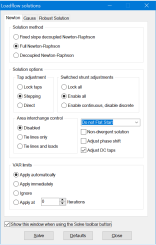
\includegraphics[scale=0.32]{fig3_loadflow.pdf}
\caption{Loadflow settings}
\label{fig:3}
\end{figure}

Check the output bar for the ``System total mismatch'' as shown in Fig. \ref{fig:4}. If the loadflow converged then the mismatch should be less than 0.01 MVA. If this is not the case then you might have repeat the loadflow until it converges.

\begin{figure}[h]
\centering
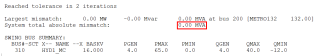
\includegraphics[scale=0.32]{fig4_mismatch.pdf}
\caption{System total mismatch}
\label{fig:4}
\end{figure}

Once the base case has been solved it is a good practice to save this as a separate file. Use the menu bar: \textbf{\textcolor{gray}{File \textgreater \phantom{ }Save As}} and called the saved case ``basecase.sav''.

\subsection{Viewing results}
One quick way to view your results is to use the spreadsheet viewer. You can examine the bus voltages and slack bus generation. We can also observe the line flows by opening the single line diagram and viewing the gauges. We will now explore how we can export the results so that they:
\begin{itemize}
\item{Won't be overwritten when you perform another load flow}
\item{Can be viewed without opening PSS/E}
\item{Easier to import into reports etc.}
\end{itemize}

To export the results, use the menu bar: \textbf{\textcolor{gray}{Power Flow \textgreater \phantom{ }Reports \textgreater \phantom{ }Bus based reports}}.  Complete the dialogue box with the following settings and press the  \textbf{\textcolor{gray}{OK}} button.

\begin{figure}[h]
\centering
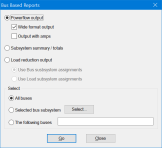
\includegraphics[scale=0.32]{fig5_report.pdf}
\caption{Bus based report dialogue}
\label{fig:5}
\end{figure}

In the output bar, a new tab called ``LOUT'' should appear. Right click on this as shown below and click \textbf{\textcolor{gray}{Save As...}}.

\begin{figure}[h]
\centering
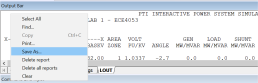
\includegraphics[scale=0.32]{fig6_lout.pdf}
\caption{Saving report to text file}
\label{fig:6}
\end{figure}


In the Save As dialogue box, name the report as ``basecase.txt''. Now you should be able to open this with a text editor (e.g. Notepad). To interpret the report, the following abbreviations may be helpful:

\begin{table}[h]
\caption{Transformer codes}
\centering
\begin{tabular}{|l|l|}
\hline
\textbf{Abbreviation} & \textbf{Meaning}                        \\ \hline
HI                    & Transformer at high tap limit           \\ \hline
LO                    & Transformer at low tap limit            \\ \hline
RG                    & Transformer controlled voltage in range \\ \hline
Un                    & Uncontrolled side                       \\ \hline
Lk                    & Taps locked                             \\ \hline
\end{tabular}
\label{table:1}
\end{table}

\begin{table}[h]
\caption{Generator codes}
\centering
\begin{tabular}{|l|l|}
\hline
\textbf{Abbreviation} & \textbf{Meaning}                                 \\ \hline
H                     & Generator at high reactive limit                 \\ \hline
L                     & Generator at low reactive limit                  \\ \hline
R                     & Generator regulating voltage (in reactive range) \\ \hline
\end{tabular}
\label{table:2}
\end{table}

\newpage
There are a couple of ways to export the diagram. One good way is to first press the ``Zoom Extent'' button on the \mychar{zoom.png} toolbar to fit the diagram onto the screen and then use the menu bar: \textbf{\textcolor{gray}{File \textgreater \phantom{ }Print...}} and choose set the printer name to ``Microsoft Print to PDF''. It will then prompt you to give a filename -- for this task name the figure ``basecase.pdf''.

Finally, if you need to export any of the spreadsheets in the spreadsheet viewer, first left click on the top left cell so the entire spreadsheet turns black, and then right click and choose ``Export active spreadsheet tab to Excel''. This procedure is shown below:

\begin{figure}[h]
\centering
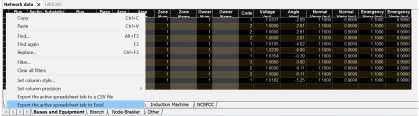
\includegraphics[scale=0.32]{fig7_excel.pdf}
\caption{Copying spreadsheet to Excel}
\label{fig:7}
\end{figure}

\subsubsection*{Activities}
\begin{enumerate}
\item[\textbf{6.2.1}] Are the network voltages within the normal operating range?
\item[\textbf{6.2.2}] Are the taps within the regulating range of the transformers?
\item[\textbf{6.2.3}] Why do the hydro generators have different power and reactive outputs?
\item[\textbf{6.2.4}] Are the line flows within the line ratings?
\end{enumerate}

\section{Effect of line outages}

\subsection{Background}
This task will put together everything we have covered so far. It is very similar to the lab for next week so it will be good practice.

In addition to studying a power system in the steady state with all lines in service, the effect of outages of lines and transformers has to be studied to determine the loading of the remaining lines and the network voltages.  Following a line outage, if voltages have changed significantly, the voltage controlling transformers will change 	their tap to restore the bus voltage within the voltage control range. The tap changing mechanism is mechanical and can take 1 -- 2 minutes to operate.  The voltages before tap changing are studied to determine whether the voltages are within the ``short term'' control range. The voltages are also determined following tap changing to determine whether the voltages can be restored to the ``normal'' control 	range.

\subsection{Procedure}
Now that we have solved the base case we can find what happens when there are line outages. Recall in Section 2, the design criteria specifies the bus voltage requirements in the event of an outage. The general procedure to conduct this study is as follows:

\begin{figure}[h]
\centering

\includegraphics[scale=0.50]{fig8_flow.pdf}
\caption{Flow chart of procedure to analyse line outages}
\label{fig:8}
\end{figure}

Observe that each iteration we need to reload the base case. Each time you perform a load flow it is a good practice to save the case with a unique (meaningful) name.

To trip a line you have two options:
\begin{itemize}
\item{Using the spreadsheet viewer, on the \textbf{\textcolor{gray}{AC Line}} tab, for the chosen line uncheck the ``In service'' check box. Remember to disappear the \mychar{pencil.png} symbol by click on a different row. This is essential to commit the change.}
\item{On the diagram viewer, right click on the chosen line and click \textbf{\textcolor{gray}{Switch}}}
\end{itemize}

\subsubsection*{Activities}
\begin{enumerate}
\item[\textbf{6.2.1}] Does the system meet the design criteria in the short term control range? (Hint: use lock taps when performing load flow.)
\item[\textbf{6.2.2}] Does the system meet the design criteria in the normal control range? (Hint: use stepping taps when performing load flow.)
\end{enumerate}


\end{document}